\def\nr{8. Aufgabenblatt}
\def\kopf{\\\hfill\normalsize\mdseries}
\documentclass[11pt,a4paper,fleqn]{scrartcl}
\usepackage{eurosym}
%\usepackage{a4kopka}
\usepackage{amsmath,amssymb,amsthm,amsfonts}
\usepackage[utf8]{inputenc}
\usepackage{algorithmic,algorithm}
\usepackage{graphics,graphicx}
\usepackage{pgfplots,tikz}
\usepackage{enumerate}
\usepackage[ngerman]{babel}
% \usepackage[software]{mymacros}
%\usepackage{matrix}
\usepackage{hyperref}
% \usepackage{caption}
\usepackage{caption, subcaption}

\floatname{algorithm}{Algorithmus}
\renewcommand{\algorithmicrequire}{\textbf{Input:}}
\renewcommand{\algorithmicensure}{\textbf{Output:}}

%\usepackage{enumitem} 
%\textheight25cm
\textheight23cm
\topmargin-15mm
\oddsidemargin-5mm    %  -10mm
\textwidth17cm    %   18.8cm
\footskip0pt
\thispagestyle{empty}
\parindent0mm
\parskip0ex
\parskip0ex

\makeatletter
\DeclareOldFontCommand{\rm}{\normalfont\rmfamily}{\mathrm}
\DeclareOldFontCommand{\sf}{\normalfont\sffamily}{\mathsf}
\DeclareOldFontCommand{\tt}{\normalfont\ttfamily}{\mathtt}
\DeclareOldFontCommand{\bf}{\normalfont\bfseries}{\mathbf}
\DeclareOldFontCommand{\it}{\normalfont\itshape}{\mathit}
\DeclareOldFontCommand{\sl}{\normalfont\slshape}{\@nomath\sl}
\DeclareOldFontCommand{\sc}{\normalfont\scshape}{\@nomath\sc}
\makeatother

% \newcommand{\cg}[1]{{\color{blue} #1}}
% \newcommand{\cb}[1]{{\color{green} #1}}
% \newcommand{\cred}[1]{{\color{red} #1}}
% \newcommand{\cc}[1]{{\color{cyan} #1}}
% \newcommand{\cm}[1]{{\color{magenta} #1}}

\newcommand{\Aufgabe}[2][]{\par\bigskip{\sf\bfseries Aufgabe #2#1:}}
%\hspace{3em}{\small(#2 point\ifthenelse{#2>1}{s}{})}}\par\smallskip}
%\newcommand\aufgabe[2][~]{\par\bigskip{\sf\bfseries Aufgabe #1
%    \hspace{3em} \ifthenelse{\equal{#2}{~}}{}{(#2)}}\par\smallskip}
\usepackage{mymacros}

\begin{document}
{\sf Universit\"at Hamburg \hfill Wintersemester 2020/21 \\ Fachbereich Mathematik \\ Dr. Matthias Voigt}
\begin{center}
\ifthenelse{\equal{\nr}{no}}{\Large\sf\bfseries \kopf}{\Large\sf\bfseries Optimierung f\"ur Studierende der Informatik -- \nr.~\kopf}
\end{center}

\renewcommand{\tilde}{\widetilde}
\renewcommand{\hat}{\widehat}
\newcommand{\ri}{\mathrm{i}}
\renewcommand{\H}{\mathsf{H}}
\newcommand{\T}{\mathsf{T}}


\subsection*{Präsenzaufgaben am 11./12.01.2021}

\Aufgabe[ (Eine Iteration im Algorithmus von Edmonds und Karp)]{P1}
% Aufgabe P-1
Schauen Sie sich die folgdende Abbildung an und denken Sie sich die Markierungen weg:
\begin{center}
 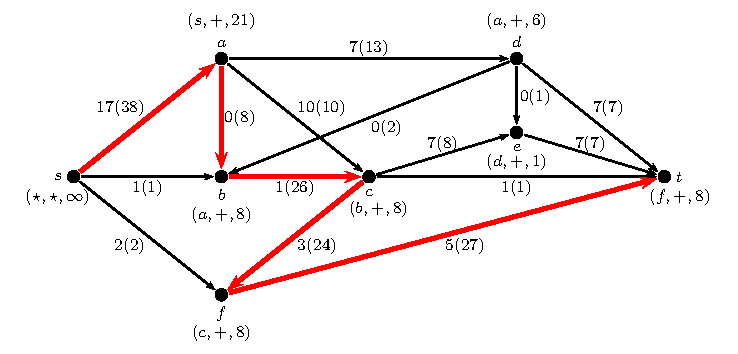
\includegraphics{fig8_1.pdf}
\end{center}

\begin{enumerate}[a)]
% Aufgabe P-1a
\item Erläutern Sie Schritt für Schritt den Markierungsprozess im Algorithmus von Edmonds und Karp: In welcher Reihenfolge wurden die Markierungen hinzugefügt und was geben die Markierungen an?

\textbf{Hinweis}: Beachten Sie zudem die übliche Regel: Gibt es mehrere Kandidaten für den nächsten zu markierenden Knoten, so ist die alphabetische Reihenfolge entscheidend.

% Aufgabe P-1b
\item Wie kommt der in der Abbildung dargestellte flussvergrößernde Pfad $(s,a,b,c,f,t)$ zustande?
% Aufgabe P-1c
\item Wie kommt der verbesserte Fluss zustande?
\end{enumerate}

\Aufgabe[ (Algorithmus von Edmonds und Karp)]{P1}
Wenden Sie den Algorithmus von Edmonds und Karp auf das folgende Netzwerk an. Gehen Sie dabei Schritt für Schritt vor, ähnlich wie im Beispiel in Vorlesung 7. Es gelte wie üblich die Regel aus Aufgabe P1.

\begin{center}
 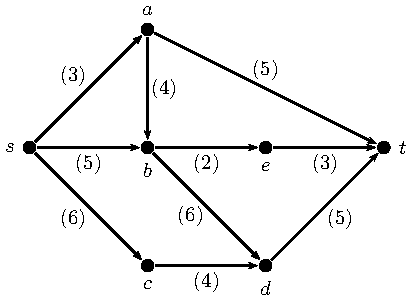
\includegraphics{fig8_2.pdf}
\end{center}



\subsection*{Hausaufgaben bis zum 20.01.2021 (12:00 Uhr)}
\emph{Bitte reichen Sie Ihre Hausaufgaben in festen Zweier- oder Dreiergruppen bei Moodle ein. Bitte laden Sie ausschließlich \textbf{PDF-Dokumente} hoch, andernfalls können Ihre Hausaufgaben nicht korrigiert werden.}

\Aufgabe[ (Algorithmus von Edmonds und Karp, 10 Punkte)]{H1}
Wenden Sie den Algorithmus von Edmonds und Karp auf das folgende Netzwerk an. Gehen Sie dabei Schritt für Schritt vor, ähnlich wie im Beispiel in Vorlesung 7. Es gelte wie üblich die Regel aus Aufgabe P1. Geben Sie auch in jeder Iteration die Knotenmarkierungen und die Warteschlange der zu untersuchenden Knoten an. Geben Sie am Ende auch einen Maximalfluss, sowie einen minimalen Schnitt an.

\begin{center}
 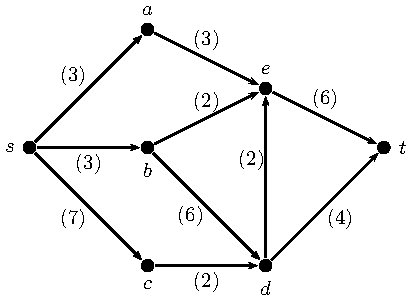
\includegraphics{fig8_3.pdf}
\end{center}

\end{document}
